\documentclass[a4paper]{article}
\usepackage[utf8]{inputenc}
\usepackage[english]{babel}
\usepackage{listings}
\usepackage[a4paper,margin=1.2in]{geometry}
\usepackage{indentfirst}
\usepackage{graphicx}
\usepackage{caption}
\usepackage{float}
\usepackage{hyperref}

\begin{document}

\title{Report: comparison of 9 global optimization methods on several test problems classes}
\author{Vladislav Sovrasov}
\date{}
\maketitle

\section{List of the algorithms}
\begin{itemize}
  \item Algorithm of global search (AGS) (\url{https://github.com/sovrasov/ags_nlp_solver})
  \item Multi Level Single Linkage (MLSL) (\url{https://nlopt.readthedocs.io/en/latest/NLopt_Algorithms/#mlsl-multi-level-single-linkage})
  \item DIRECT (\url{https://nlopt.readthedocs.io/en/latest/NLopt_Algorithms/#direct-and-direct-l})
  \item Locally-based DIRECT (DIRECT$l$) (\url{https://nlopt.readthedocs.io/en/latest/NLopt_Algorithms/#direct-and-direct-l})
  \item Dual Simulated Annealing (\url{https://github.com/sgubianpm/sdaopt})
  \item Differential Evolution (\url{https://docs.scipy.org/doc/scipy/reference/generated/scipy.optimize.differential_evolution.html#scipy.optimize.differential_evolution})
  \item Controlled Random Search (\url{https://nlopt.readthedocs.io/en/latest/NLopt_Algorithms/#controlled-random-search-crs-with-local-mutation})
  \item Simple (\url{https://github.com/chrisstroemel/Simple})
  \item StoGO (\url{https://nlopt.readthedocs.io/en/latest/NLopt_Algorithms/#stogo})
\end{itemize}

All parameters of the methods can be found in \textit{experiments/solve\_different\_methods.py} script.
Since NLOpt hasn't an API to control parameters of the algorithms from Python, it was built with $\varepsilon=10^{-4}$ for DIRECT and DIRECT$l$ methods.

\section{List of the test problems}

\begin{itemize}
  \item Functions from $F_{GR}$ class. It consists of 100 multi-extremal problems of the same structure. The description can be found in \url{https://core.ac.uk/download/pdf/82313177.pdf}.
  \item Functions from classes generated by the GKLS generator (\url{http://wwwinfo.deis.unical.it/yaro/GKLS.html}).
\end{itemize}

Each class consists of 100 multi-extremal problems with 10 and more local minima. Problem is considered solved when optimization method placed a new trial point in the $\Delta$-vicinity of the known global optima $x^*$: $\Vert x^* - \widetilde{x} \Vert_{\inf} \le \Delta$.


\section{Results on the $F_{GR}$ class}

\begin{figure}[H]
  \center
  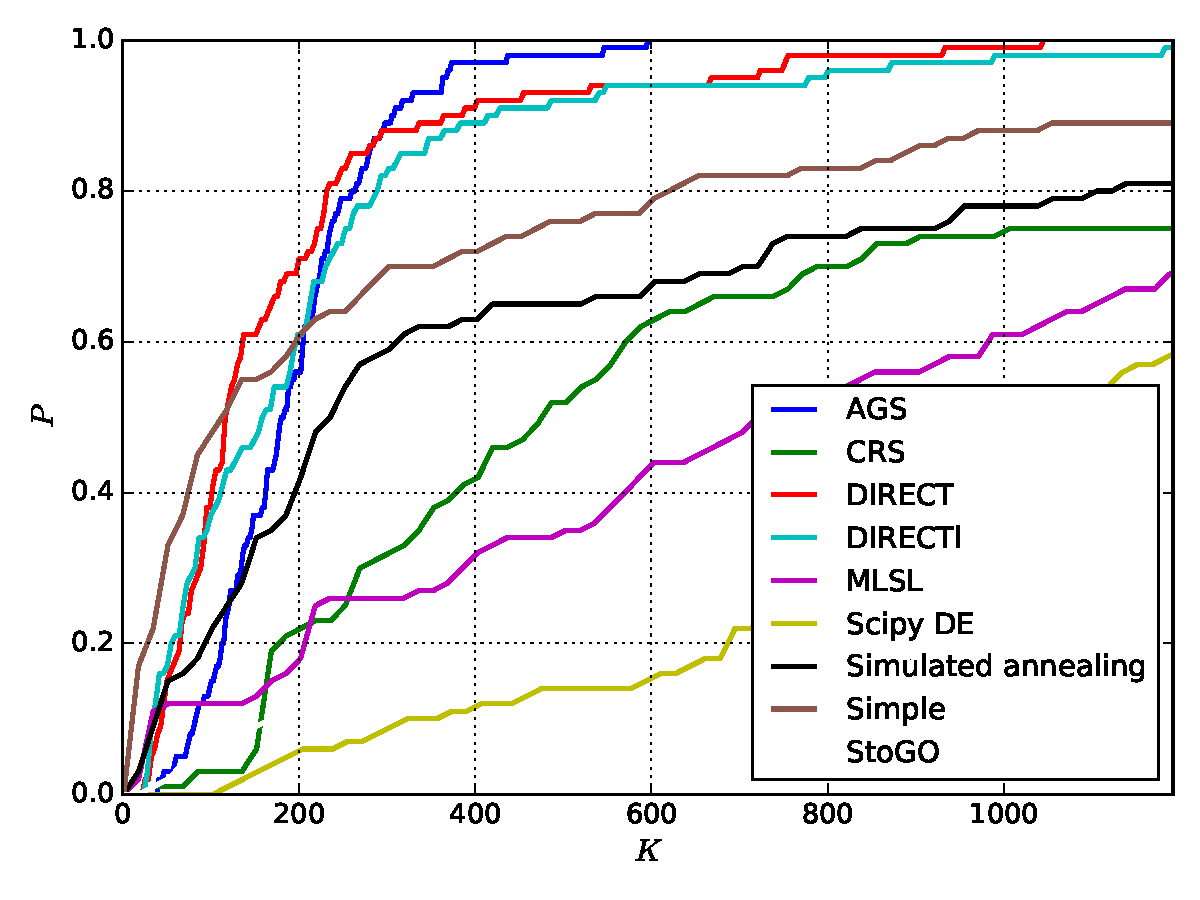
\includegraphics[width=0.95\textwidth]{../experiments/grish/cmc.pdf}
  \caption{$\Delta=10^{-2}$}
\end{figure}

%table grish

\section{Results on the $GKLS$ problems}

\begin{figure}[H]
  \center
  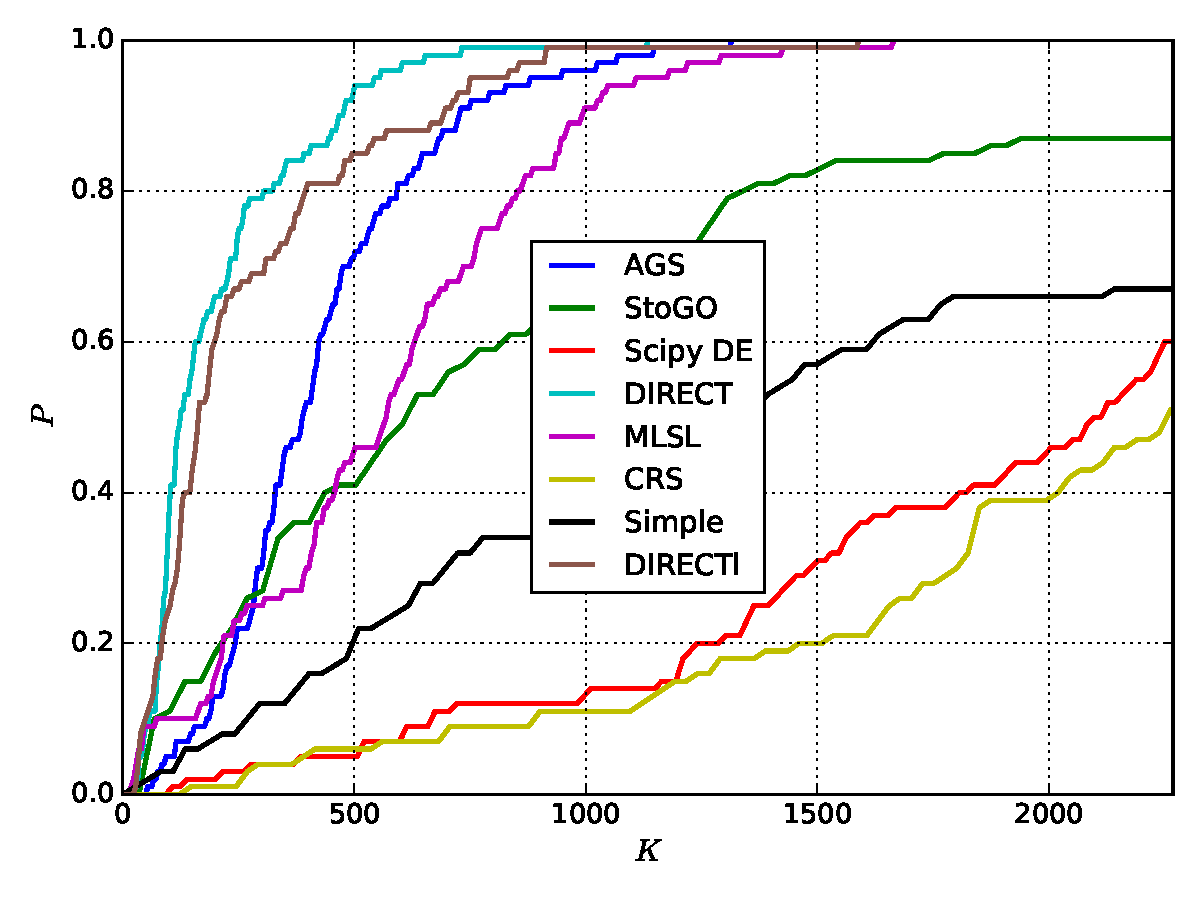
\includegraphics[width=0.95\textwidth]{../experiments/gklss2d/cmc.pdf}
  \caption{Class GKLS Simple 2d. $\Delta=2\cdot10^{-2}$}
\end{figure}

%table gklss2d

\begin{figure}[H]
  \center
  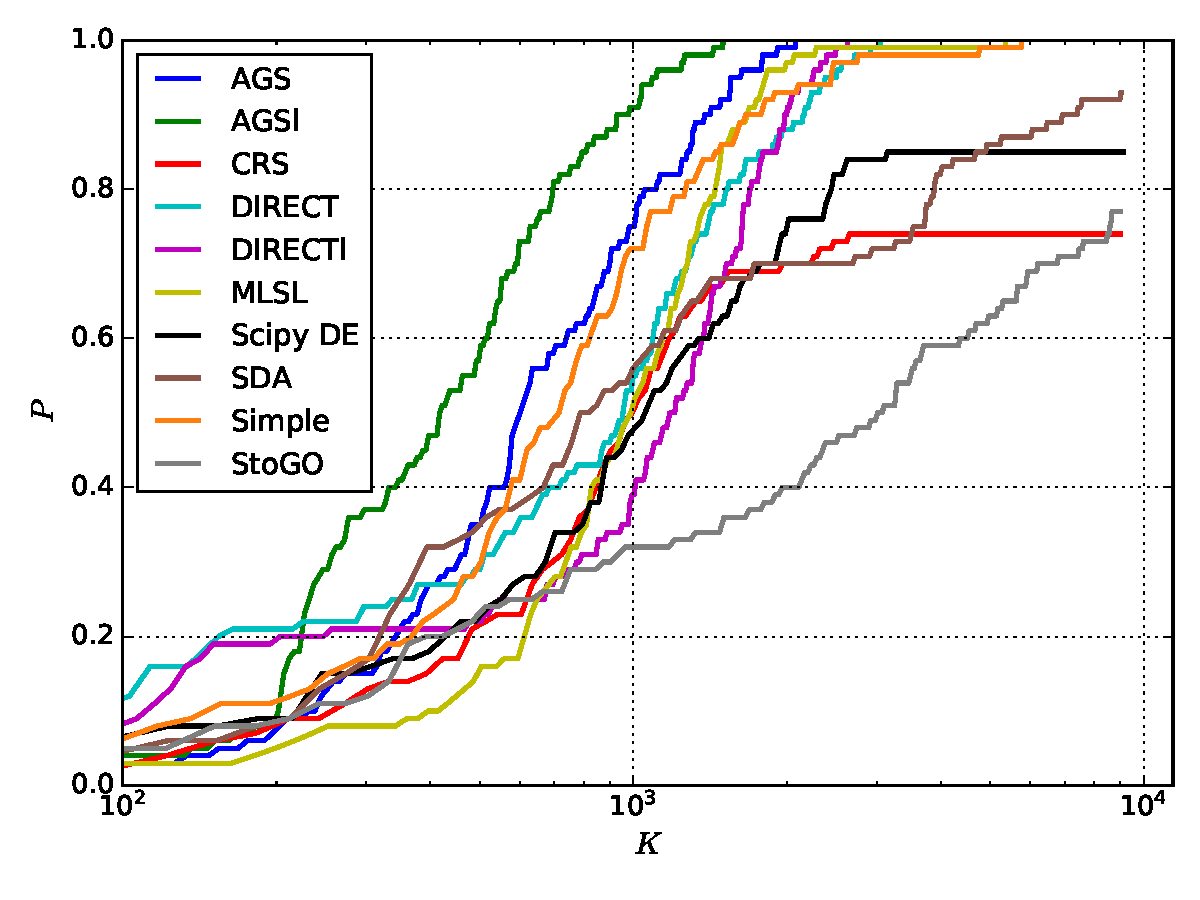
\includegraphics[width=0.95\textwidth]{../experiments/gklsh2d/cmc.pdf}
  \caption{Class GKLS Hard 2d. $\Delta=2\cdot10^{-2}$}
\end{figure}

%table gklsh2d

\begin{figure}[H]
  \center
  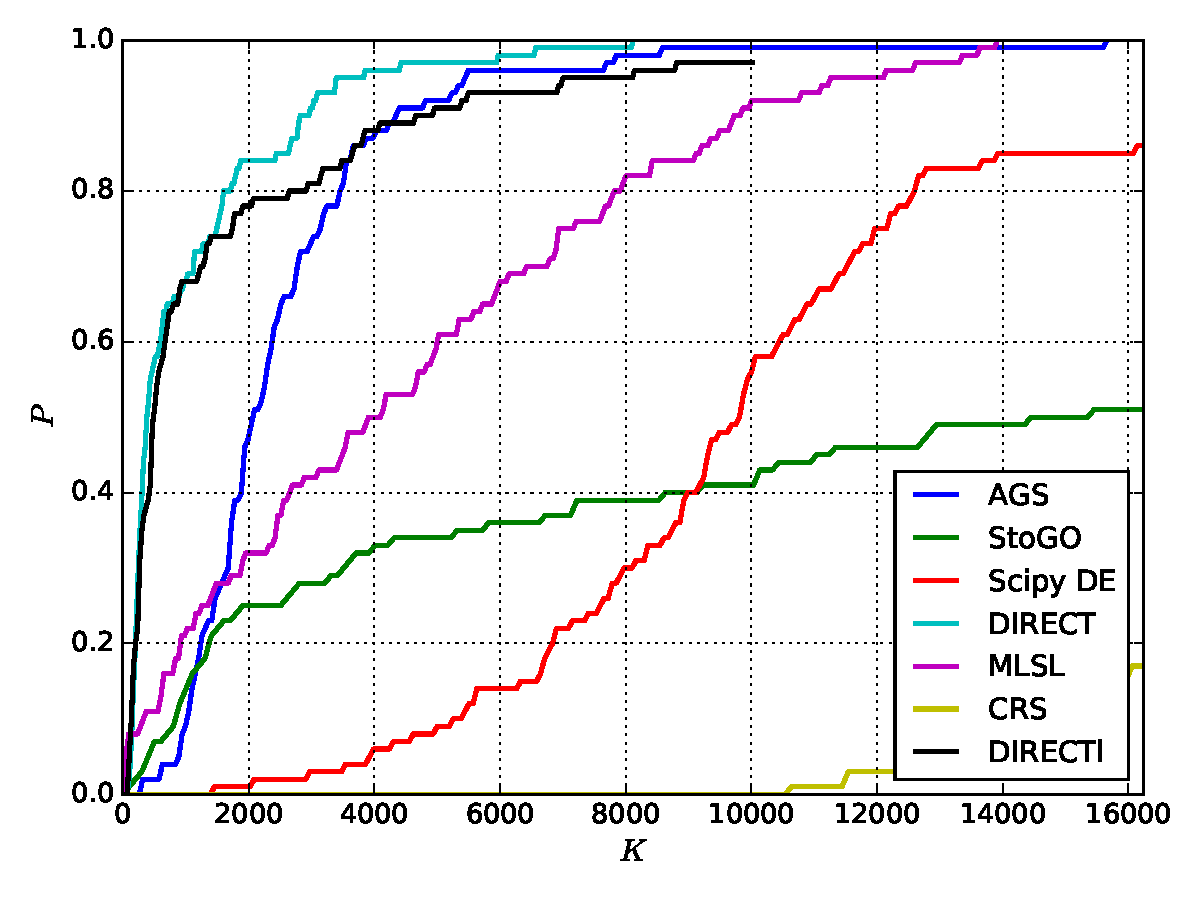
\includegraphics[width=0.95\textwidth]{../experiments/gklss3d/cmc.pdf}
  \caption{Class GKLS Simple 3d. $\Delta=2\cdot10^{-2}$}
\end{figure}

%table gklss3d

\begin{figure}[H]
  \center
  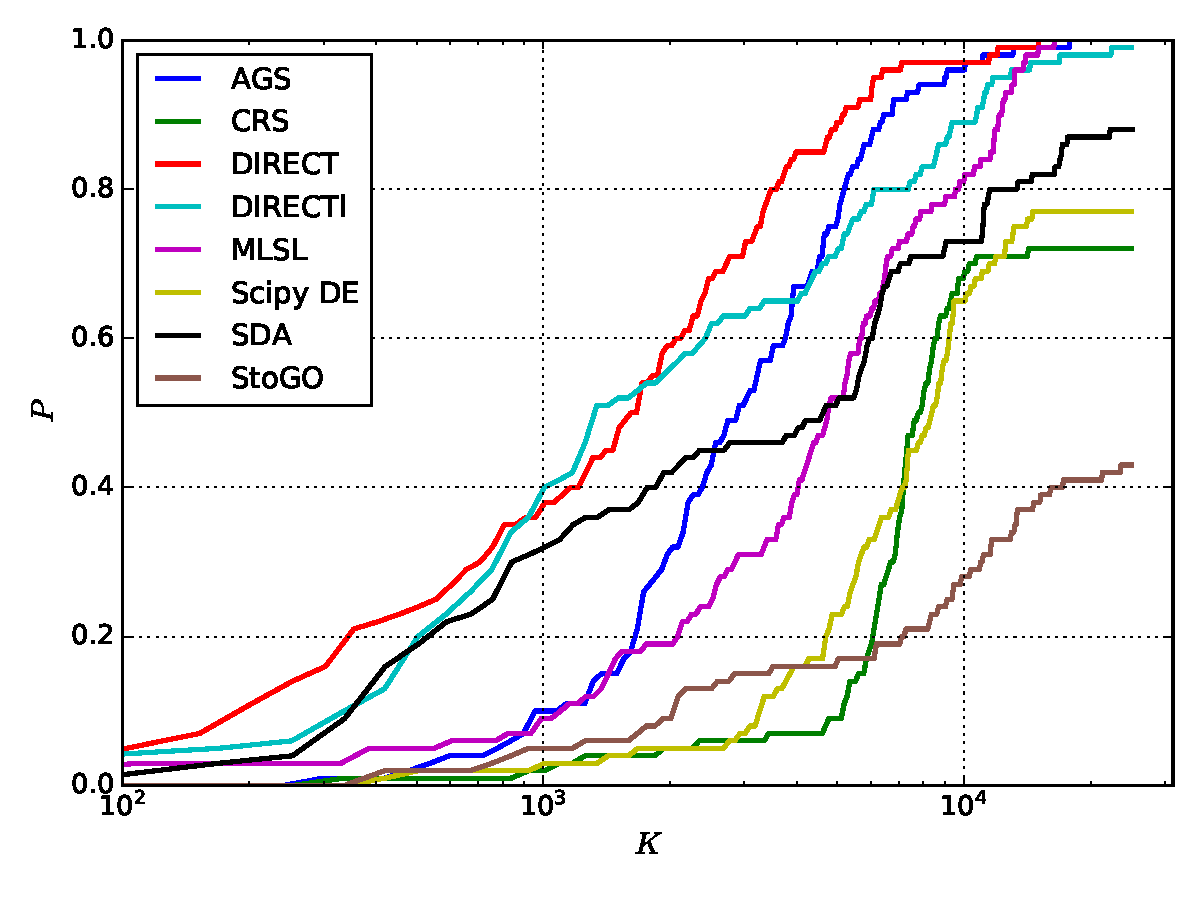
\includegraphics[width=0.95\textwidth]{../experiments/gklsh3d/cmc.pdf}
  \caption{Class GKLS Hard 3d. $\Delta=2\cdot10^{-2}$}
\end{figure}

%table gklsh3d

\begin{figure}[H]
  \center
  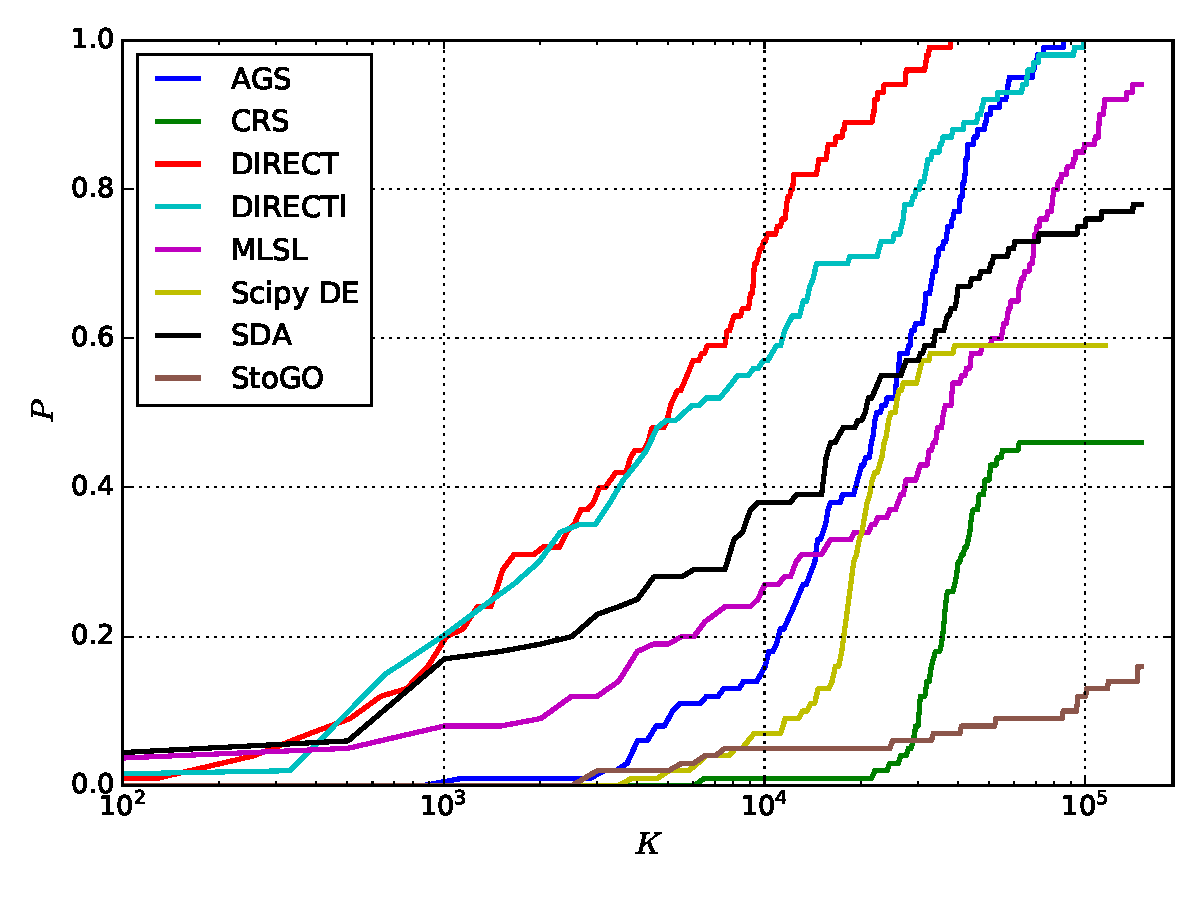
\includegraphics[width=0.95\textwidth]{../experiments/gklss4d/cmc.pdf}
  \caption{Class GKLS Simple 4d. $\Delta=2\cdot10^{-2}$}
\end{figure}

%table gklss4d

\begin{figure}[H]
  \center
  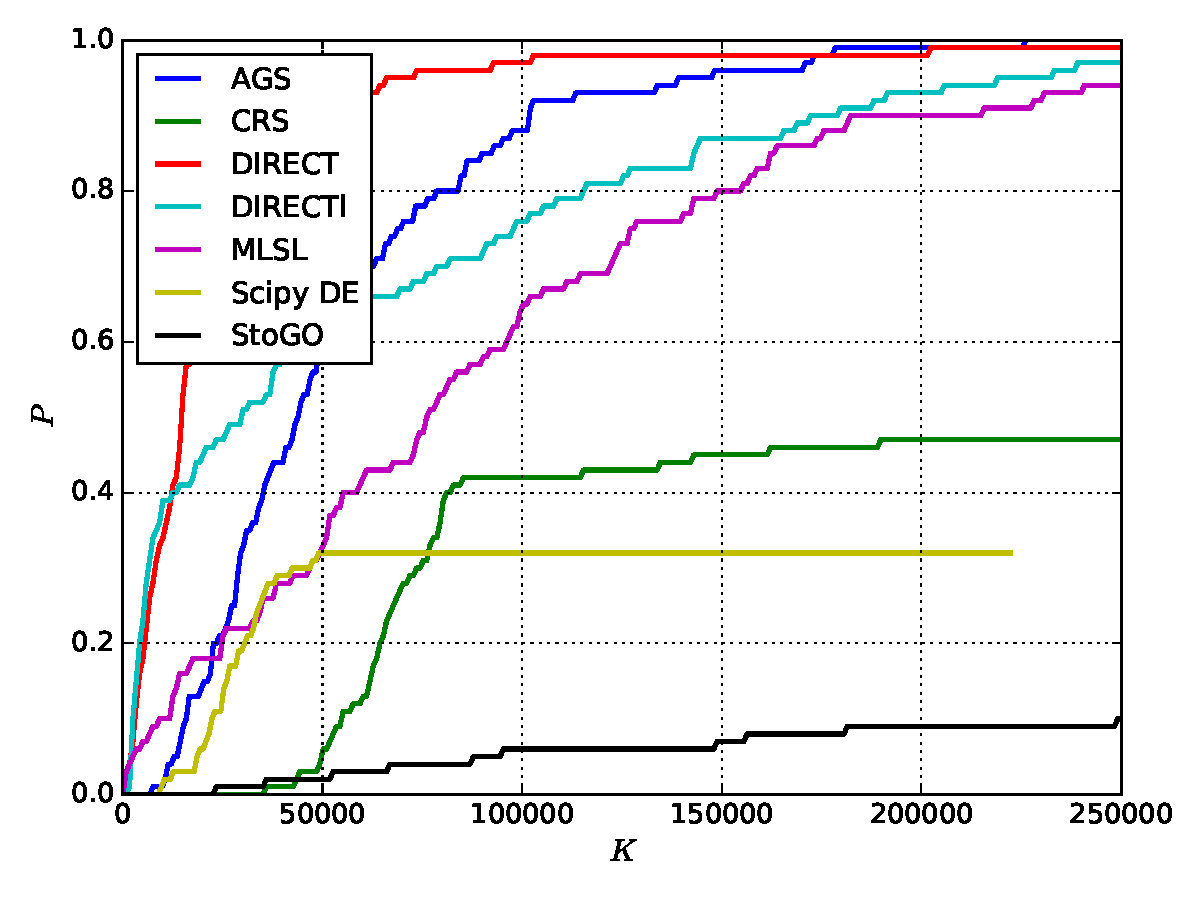
\includegraphics[width=0.95\textwidth]{../experiments/gklsh4d/cmc.pdf}
  \caption{Class GKLS Hard 4d. $\Delta=2\cdot10^{-2}$}
\end{figure}

%table gklsh4d

\begin{figure}[H]
  \center
  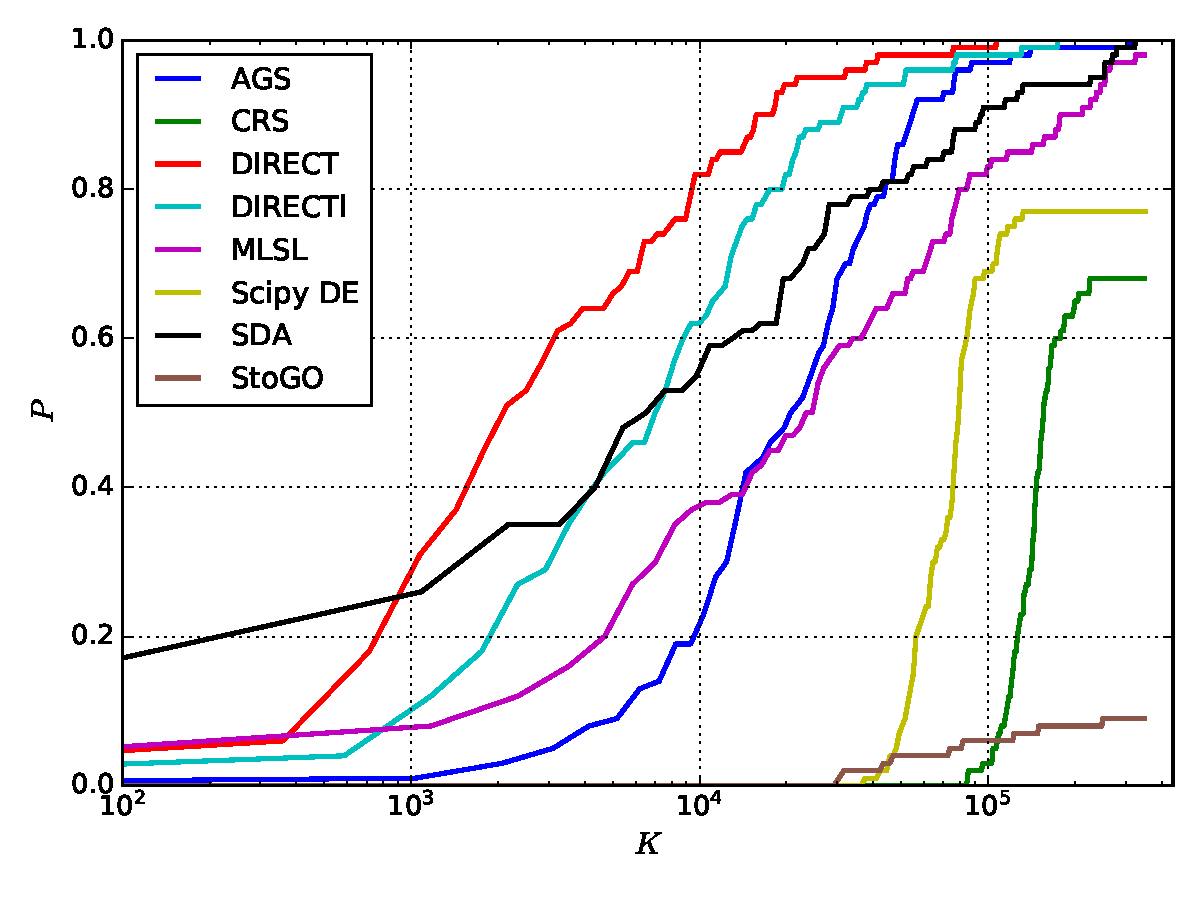
\includegraphics[width=0.95\textwidth]{../experiments/gklss5d/cmc.pdf}
  \caption{Class GKLS Simple 5d. $\Delta=2\cdot10^{-2}$}
\end{figure}

%table gklss5d

\begin{figure}[H]
  \center
  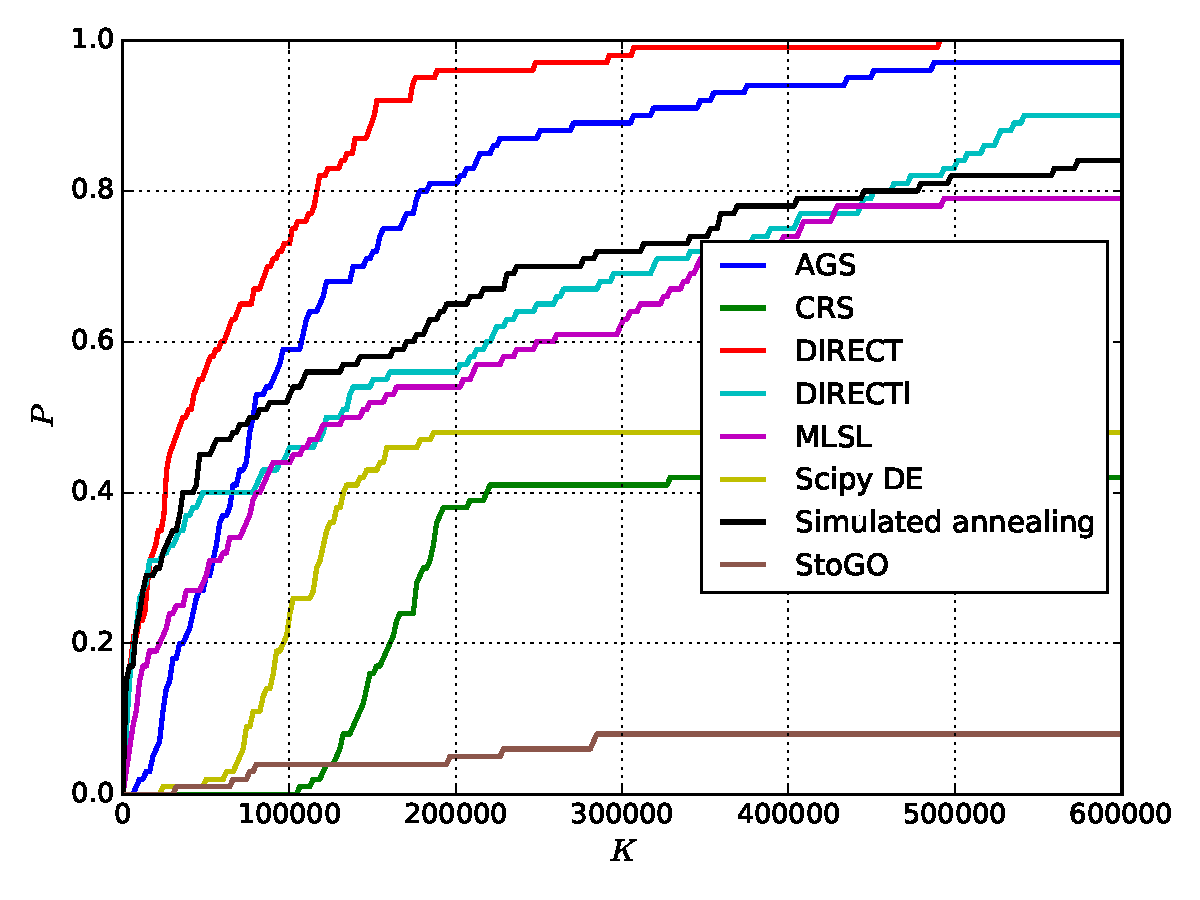
\includegraphics[width=0.95\textwidth]{../experiments/gklsh5d/cmc.pdf}
  \caption{Class GKLS Hard 5d. $\Delta=2\cdot10^{-2}$}
\end{figure}

%table gklsh5d

\begin{figure}[H]
  \center
  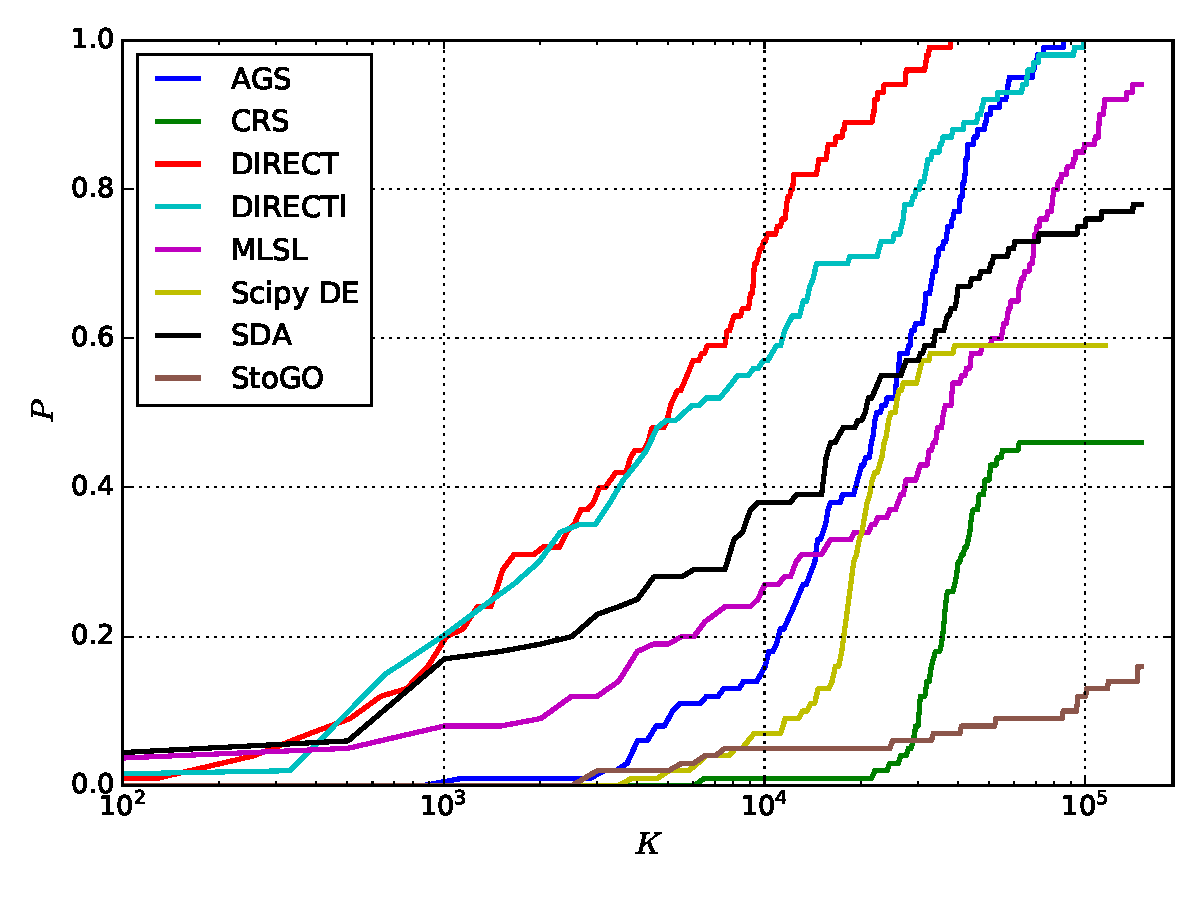
\includegraphics[width=0.95\textwidth]{../experiments/gklss4d/cmc.pdf}
  \caption{Class GKLS Simple 4d. $\Delta=0.0632$}
\end{figure}

%table gklss4d_serg

\begin{figure}[H]
  \center
  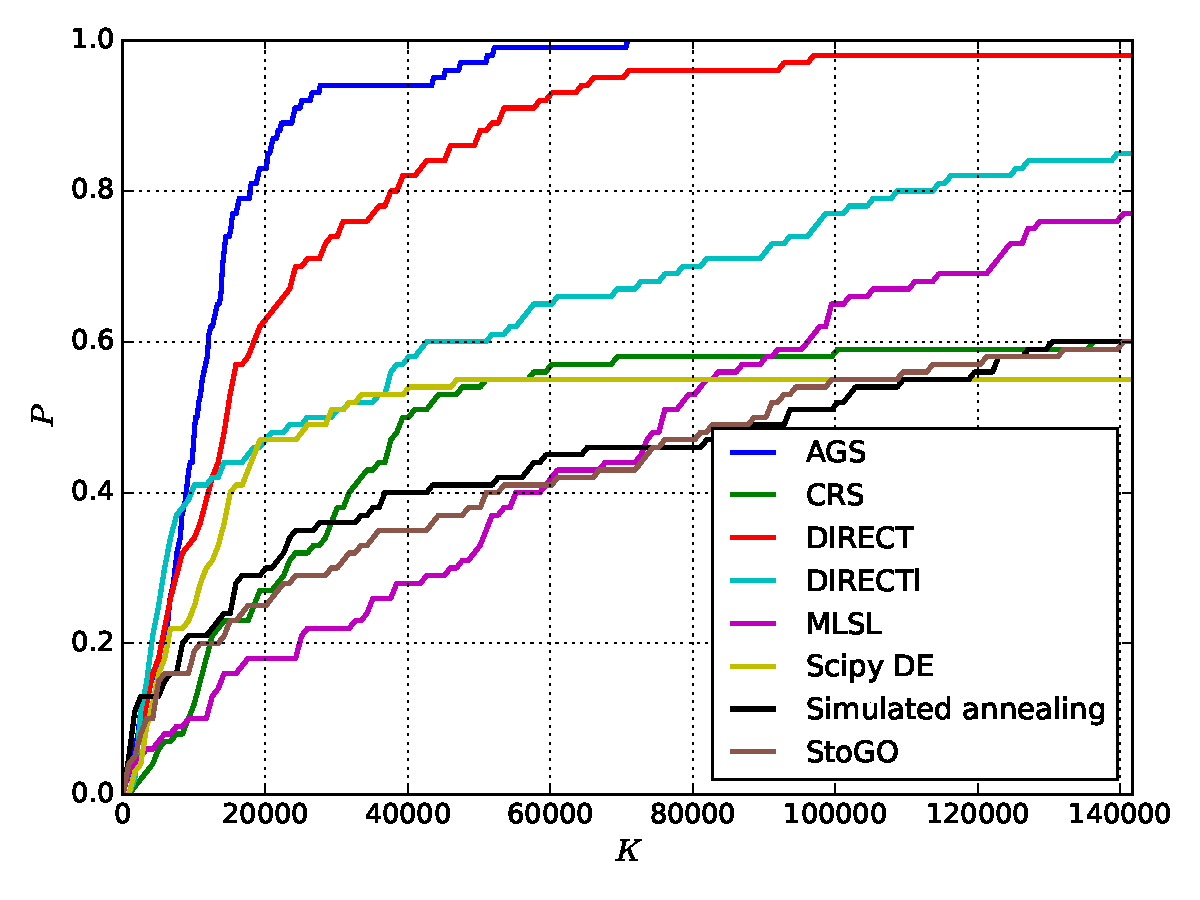
\includegraphics[width=0.95\textwidth]{../experiments/gklsh4d_serg/cmc.pdf}
  \caption{Class GKLS Hard 4d. $\Delta=0.0632$}

\end{figure}

%table gklsh4d_serg

\begin{figure}[H]
  \center
  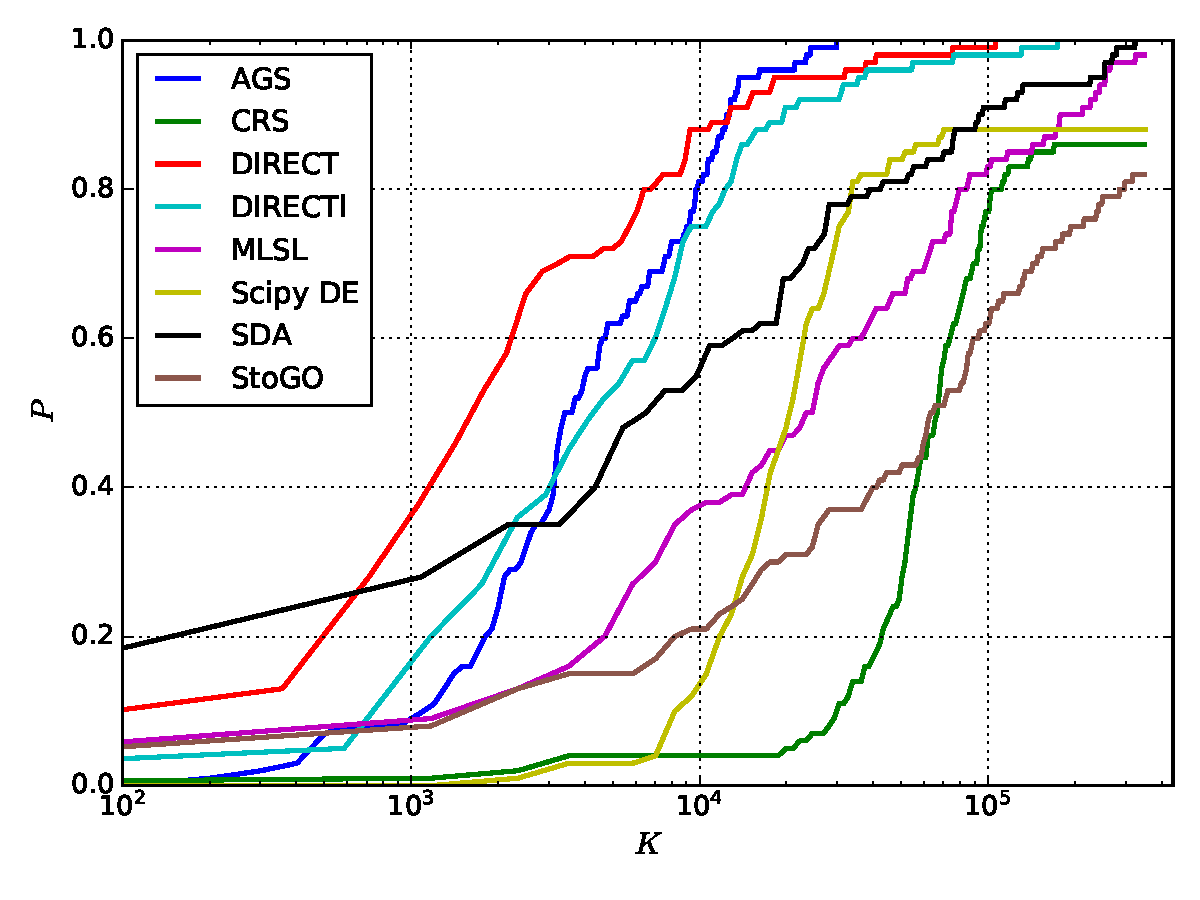
\includegraphics[width=0.95\textwidth]{../experiments/gklss5d_serg/cmc.pdf}
  \caption{Class GKLS Simple 5d. $\Delta=0.0796$}

\end{figure}

%table gklss5d_serg

\begin{figure}[H]
  \center
  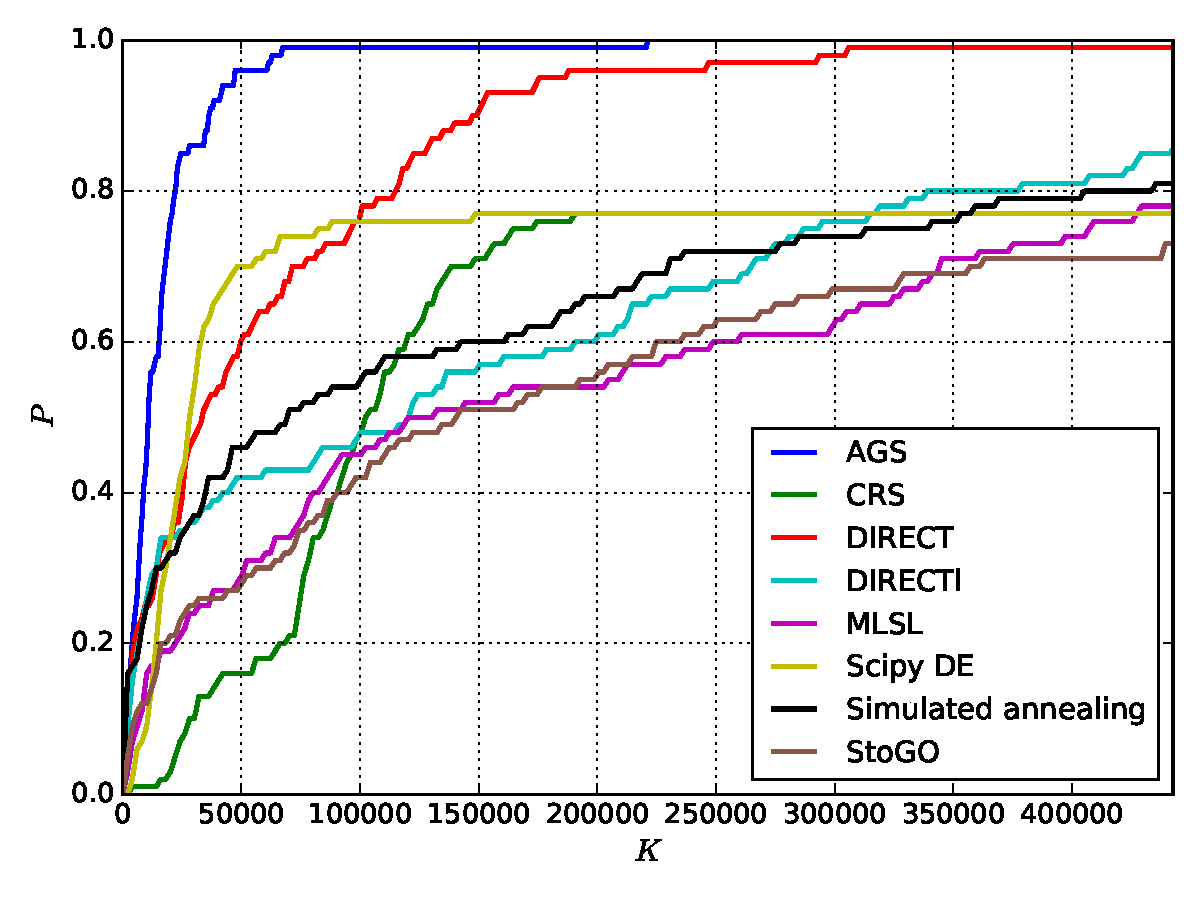
\includegraphics[width=0.95\textwidth]{../experiments/gklsh5d_serg/cmc.pdf}
  \caption{Class GKLS Hard 5d. $\Delta=0.0796$}

\end{figure}

%table gklsh5d_serg

\end{document}
